\documentclass[twoside]{report}
\usepackage{todonotes}
\usepackage{hyperref}
\usepackage[backend=biber, style=numeric-comp, sorting=none]{biblatex}
\addbibresource{references.bib}

\title{Labbook graduation-project Lex Bolt}
\date{\today}

\begin{document}

\chapter*{Labbook research Lex Bolt}

\section*{Introduction}
This project studies the research question 'Generating bird’s eye view images to estimate team positions'.

\section*{5 June}
Bot the ViT and CCT transformer based models performed really poorly on my dataset. It could be because of the untuned hyper parameters but I do not think I have enough time left to fine-tune those. I also tried the new Lion optimiser, which should have the state-of-the-art performance.

\section*{3 June}
Currently training CCT model, which is a transformer based model that makes use of convolutions to see if it can maybe produce better results than GoogLeNet. 

\section*{2 June}
Reworked the python script to match the images to the optitrack data to take advantage of the increased accuracy of the rigid body recording.

The model gives an average distance of 20.3 from the predicted location to the true location.
This is better than the expected average distance from two randomly chosen points on a rectangle, which in this case is 45.92.
The formula to calculate the average expected distance between two points on a rectangle with dimensions (90, 60), where $a \geq b$ is \cite{avgdistance}: 

\begin{equation}
a(X) = \frac{1}{15} \left(\left( \frac{a^3}{b^2} + \frac{b^3}{a^2}\right) + \sqrt{a^2 + b^2} \left(3 - \frac{a^2}{b^2} + \frac{b^2}{a^2}\right)\right) + \frac{1}{6}\left(\frac{b^2}{a} ln\left(\frac{a + \sqrt{a^2 + b^2}}{b}\right) + \frac{a^2}{b}ln\left(\frac{b + \sqrt{a^2 + b^2}}{a}\right)\right)
\end{equation}
% $a(X) = \frac{1}{15}((\frac{a^3}{b^2}+\frac{b^3}{a^2}+$

\section*{1 June}
Recorded a new real-world dataset with optitrack. This time selecting the markers I wanted to track and create a rigid body from them. This makes sure there are 0 false positives in the real-world dataset, giving me a much greater accuracy.

\section*{31 May}
Tried matching and evaluating the model on the real world dataset. Did not really work as there were a lot of false-positives in the dataset from random interference markers. 

\section*{30 May}
Wrote a python script that can convert the OptiTrack data to the coordinate system that I use and save it with the corresponding image from the real robot's camera. When it is done running I will manually verify the results and then I can evaluate the trained model on real-world data.

The dataset somewhat works but I will record a new one tomorrow just to be sure.

\section*{29 May}
Got python files from Nuno to extract the coordinate data from the OptiTrack recording. I am currently working on matching the recorded images from the robot's camera to the recorded coordinates.
The coordinates also do not match up as expected to the coordinate frame of the football field. I currently think that is because the OptiTrack exported coordinates are in meters, whereas the Motive coordinate system is in millimeters. 

\section*{26 May}
Recorded a real-world dataset with OptiTrack.

\section*{25 May}
Made a notebook that plots the loss and accuracy during the model's training stage. \todo{Nice training curve, but an accuracy of 50\% seems to indicate overfitting. Or is it the 50/50 error of a dihedral symmetric field? }
\begin{figure}[!h]
\begin{centering}
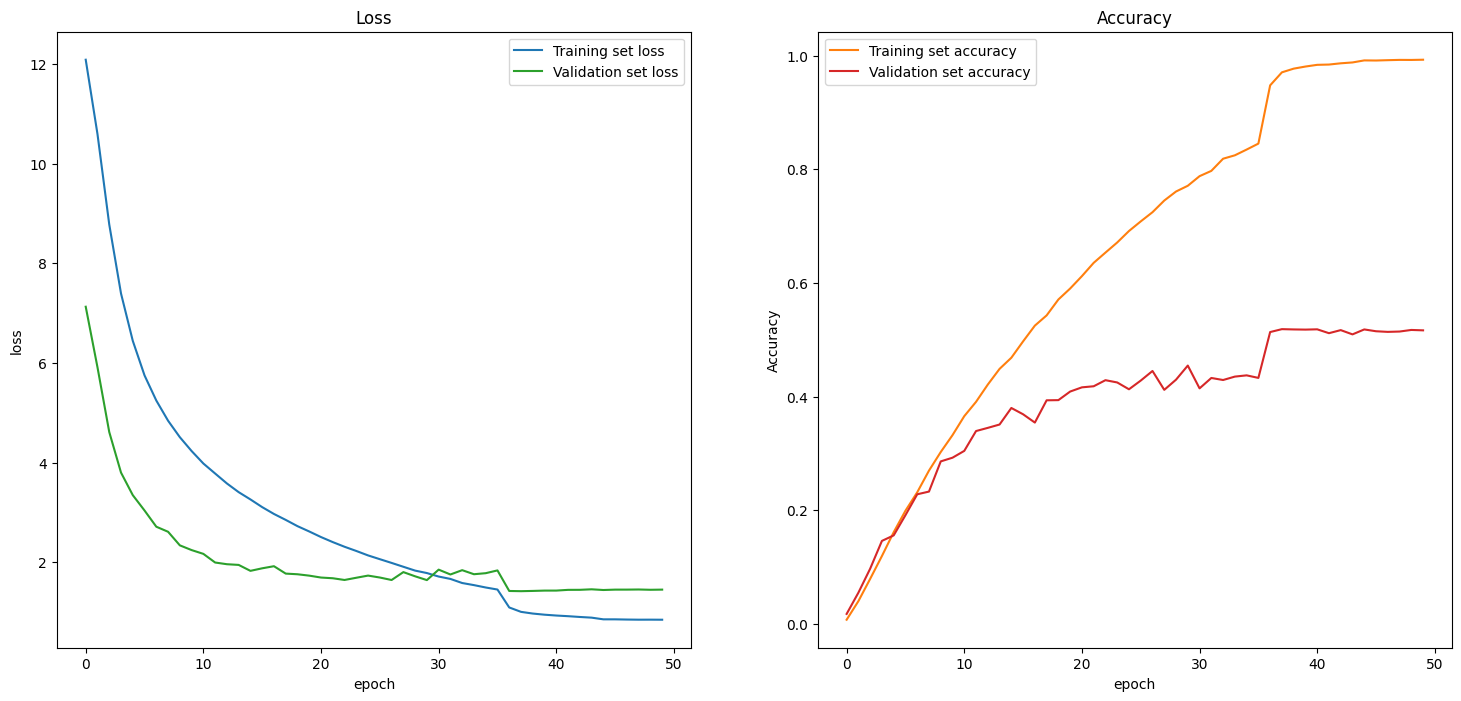
\includegraphics[width=1\textwidth]{Scriptie/imgs/isthisloss.png}
\caption{Loss and accuracy for the training of a dataset with 100.000 samples}
\end{centering}
\end{figure}

\section*{24 May}
Made a notebook to plot the predicted location next to the true location of a validation image. It plots the 10 best scoring predictions as a heatmap (indicating confidence) next to the true position. I am surprised it is not mirrored.
\begin{figure}[!h]
\begin{centering}
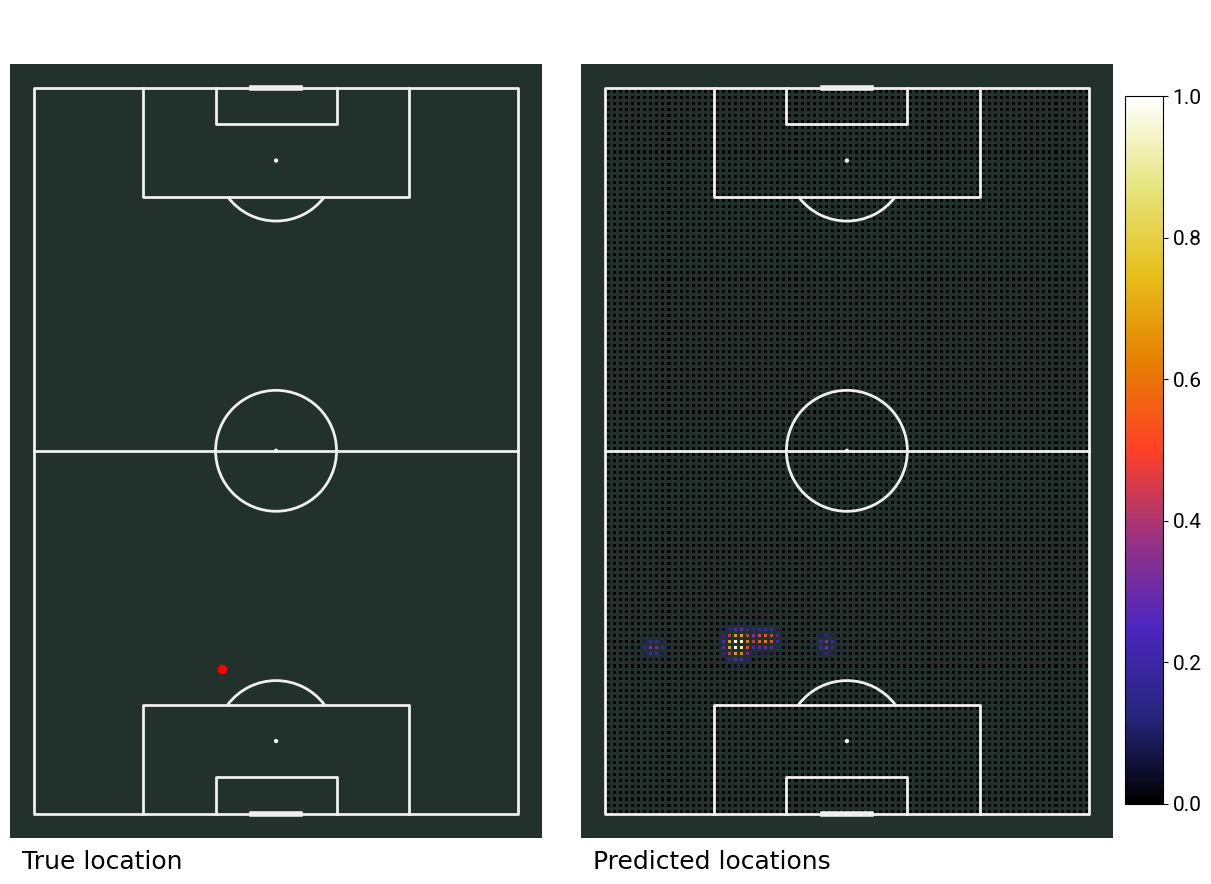
\includegraphics[width=0.9\textwidth]{Scriptie/imgs/pred.png}
\caption{true prediction (left) next to estimated position (right)}
\end{centering}
\end{figure}
\begin{figure}[!h]
\begin{centering}
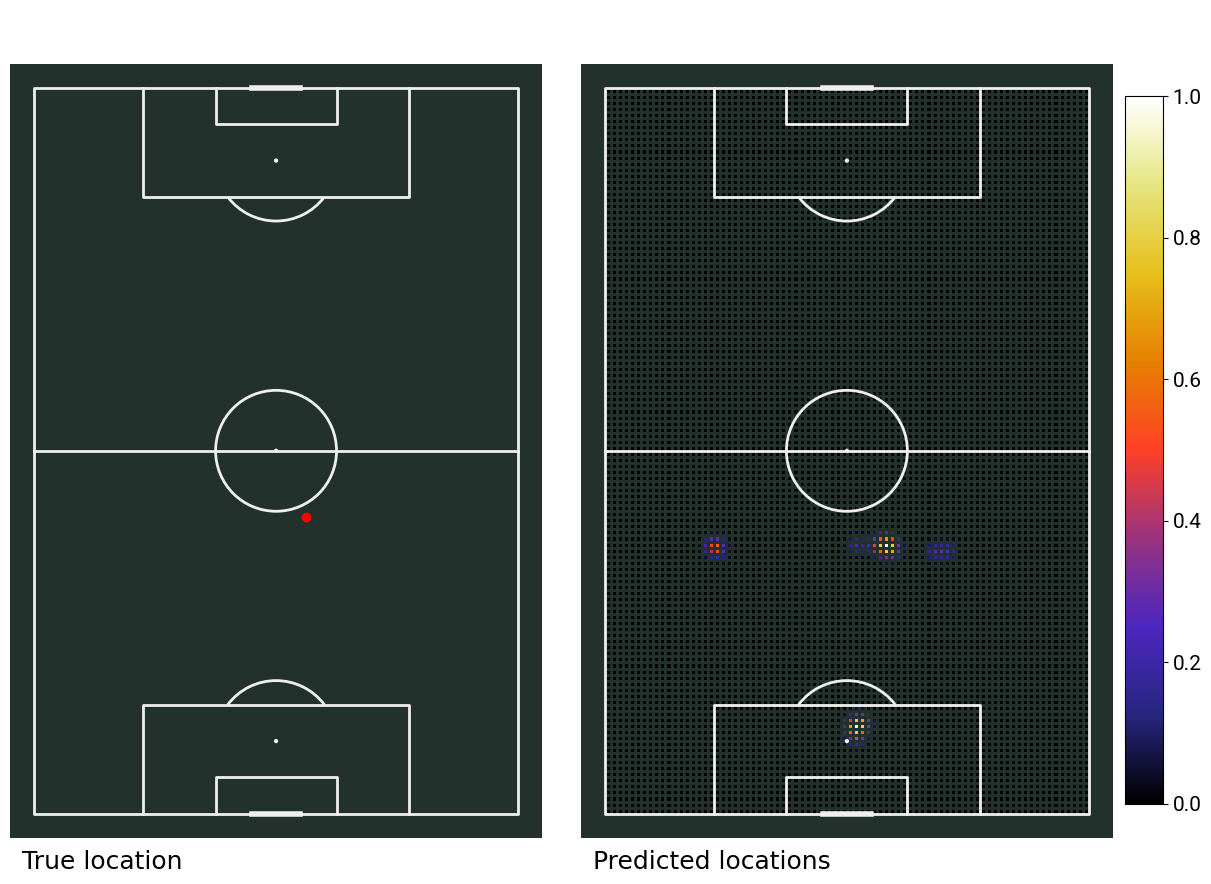
\includegraphics[width=0.9\textwidth]{Scriptie/imgs/interestingyes.png}
\caption{true prediction (left) next to estimated position (right)}
\end{centering}
\end{figure}
\hfill \break \\
I also find this one really interesting. I guess it recognised the penalty stip as well as the center dot and the curve of the penalty area that looks like the curve of the center. Maybe it learned to look at the white lines?

\section*{23 May}
Trained the model with the correct number of classes on 50 epochs. The training set fitted 99.29\% and the validation set 51.65\%. \todo{That sounds like overfitting} Note that the model only accepts a prediction as correct when it EXACTLY matches the location on the football field.

fixed a bug where the model could only use 46 instead of the 4185 classes (locations of the football field). After training for 27 epochs on the updated code it fitted 77\% on the training set and 41\% on the validation set. \todo{Still a large gap. How does the learning curve looks like? Do you train to long? Could you use some overfitting tricks to reduce this gap? Like data-augmentation, dropout, etc}


\section*{22 May}
Trained GoogLeNet on a dataset with 100.000 images (80.000 for training, 10.000 for validation and 10.000 for testing). This resulted in a training set accuracy of 98\% and a validation accuracy of 78\%.

Made some improvements to speed up the training process. Made the indexing of the dataset savable to a JSON file (360 minutes to 0.1 seconds speedup) and added the ability to save a trained model to a .pt file.
\hfill \break \\
The dataset previously loaded the RGB images as RGBA images. This could be a possible solution to the problem with the Lift-Splat-Shoot algorithm. GoogLeNet also did not like the RGBA images and gave a similar warning as the Lift-Splat-Shoot algorithm, only with more readable information.

\section*{21 May}
Implemented GoogleNet\footnote{https://paperswithcode.com/method/googlenet} to determine the position an image was taken on the football field. The test-run gave an accuracy of 98\% on the training set, showing that the model can be fitted to the dataset. Because I only used 200 samples for the first run, the validation accuracy was 2\%. I am going to train it tomorrow when I am not at home on a dataset with 100.000 samples and 50 epochs.
\begin{figure}[!h]
\begin{centering}
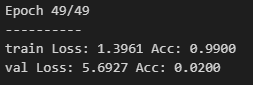
\includegraphics[scale=0.61]{Scriptie/imgs/99.png}
\caption{Training run with 200 samples}
\end{centering}
\end{figure}

\section*{17 May}
saving some papers about prediction position from a camera perspective \newline
\href{https://vciba.springeropen.com/articles/10.1186/s42492-018-0008-z}{localisation with camera} \\
\href{https://arxiv.org/abs/1709.08429}{DeepVO: Towards End-to-End Visual Odometry with Deep Recurrent Convolutional Neural Networks} \\
\href{https://arxiv.org/pdf/2212.13105.pdf}{SuperGF: Unifying Local and Global Features for Visual Localization} \\

\section*{16 May}
The authors responded: Thank you for your question! post\_rot and post\_trans are for data augmentation. They don't come from a dataset, they are randomly sampled. You can see an example of how to sample them in this line: \url{https://github.com/nv-tlabs/lift-splat-shoot/blob/master/src/data.py#L140}.

\textbf{If you don't want to use data augmentation, you can set post\_rot to an identity matrix and post\_trans to a zero vector.}
\hfill \break \\
Still getting the same error message as before. 


\section*{15 May}
Found a very promising \href{https://kth.diva-portal.org/smash/get/diva2:1335815/FULLTEXT01.pdf}{paper} that also tries to guess the location of an object on a football field, namely the ball. The approach involves training a CNN on a dataset of 2D images and corresponding 3D positions of the objects in those images. The CNN learns to map the 2D image features to the 3D position of the object.
I already have a dataset of 2D images with 3D coordinates. However, this paper focuses on getting the 3D coordinates of an object in an image, whereas I want the 3D coordinates of the camera taking the image. 
\hfill \break \\
Found a \href{https://arxiv.org/pdf/2110.00966.pdf}{paper} (\href{https://github.com/avishkarsaha/translating-images-into-maps}{code}) that proposes an alternative method to generate a Birds-Eye-View. This paper approaches it as a translation problem. They show how a novel form of transformer network can be used to map from images and video directly to an overhead map or bird’s-eye-view of the world, in a single end-to-end network. I have a feeling this paper might be a little too experimental but I can give it a try. After inspecting the code I think that this implementation would need a lot of tweaking before I can add my own dataset to it because it is very hard coded to work with NuScenes and the code style is horrendous. 
\hfill \break \\
Arnoud suggested the \href{https://arxiv.org/pdf/2305.04205.pdf}{paper} (\href{https://github.com/lynn-yu/Bi-Mapper}{code}) paper. This paper proposes Bi-Mapper. Bi-Mapper uses a combination of both top-down and bottom-up information to create a bird's eye view perspective. It builds on top of the other papers that use a front-view transformer. Sadly, the code has not yet been published. The github has only been created 5 days ago.
\hfill \break \\
Contacted Leo Dorst about the issues I am having with the matrices of the Lift-Splat-Shoot algorithm and he is willing to help. 
I e-mailed the authors of the paper with the question if they can explain the matrices to me further. 

\section*{3 May}
\begin{itemize}
    \item Meeting with Arnoud:
    \begin{itemize}
        \item For the first draft I can explain my approach, the problems I encounter and the possible ways to solve these problems.
        \item Explore other options that can generate a birds eye view perspective. The Lift-Splat-Shoot paper mentions other implementations.
        \item Could contact Leo with the question about the meaning of the post\_trans and post\_rot matrices. 
    \end{itemize}
\end{itemize}

\section*{2 May}
Tried copying and hardcoding a post\_trans and post\_rot matrix from the Nuscenes dataset into my own dataset but even this gave errors. The same shape [...] is invalid for input of size N. I also tried leaving them None or shape (0,) as the paper presents the algorithm as invariant to the number of camera's, but this also gave errors.
\newline
Tried Arnoud's suggestion to make the Post\_rot matrix and Post\_trans matrix orthogonal matrices but I still keep getting the following error: "RuntimeError: shape '[1, 4, 1, 1, 1, 3]' is invalid for input of size 16". \todo{Check your input. Is this a matrix of 16x16 or 4x4. If 4x4, where is the shape of 1x6 coming from. Try to make it a vector of 1x4}

\section*{1 May}
Spent the whole day trying to get the correct shapes for the parameters listed below. I do not know how to get the post\_rot and post\_trans matrices correct. I have the intrinsic, extrinsic, rotation and translation matrices. I have tried looking for reference material online but I can not find anything mentioning the post-rotation or post-transformation matrices. The paper about the Lift-Splat-Shoot algorithm also does not mention these matrices.
%\newline

\bigskip
Converted the rotation matrix and location matrix from the Unity perspective plugin into the extrinsic camera matrix. The rotation is stored as a quaternion so that had to be converted to a regular rotation matrix first. 


\section*{30 April}
This code is related to the translation part of the model: 
        \begin{figure}[!hbt]
        \begin{centering}
        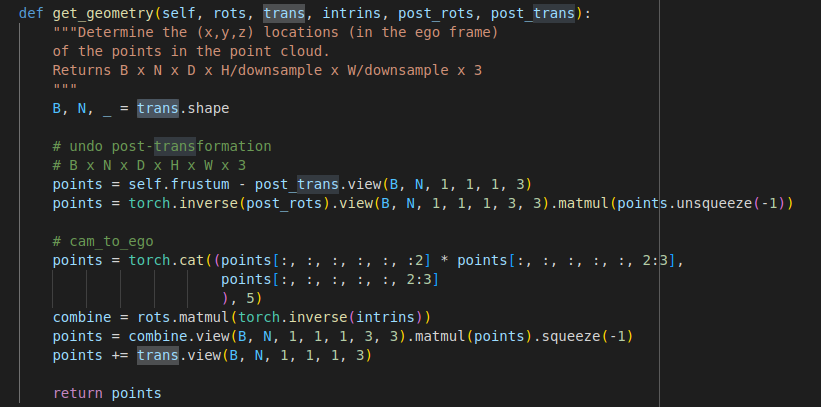
\includegraphics[scale=0.31]{Scriptie/imgs/trans.png}
        \caption{Code that undoes the post-transformation}
        \end{centering}
        \end{figure} 
        
%        \newline
I can investigate if I can remove the dependency on the transformation matrix since I am not doing any transformations on my images. The original NuScenes dataset uses 4x4 matrices for this parameter. I can not simply make them all zeros 
\todo{it is a homogeneous matrix, so element (4,4) has to stay 1.o. Have you seen this \href{https://stackoverflow.com/questions/28075743/how-do-i-compose-a-rotation-matrix-with-human-readable-angles-from-scratch/28084380#28084380}{stackoverflow answer}
?}
as it needs to be an invertible matrix\newline

\bigskip Wrote custom Dataset and Dataloader classes that are compatible with Pytorch (tested and works). These two classes contain the data in the dataset in such a way that pytorch can train the Lift-Splat-Shoot model. The only remaining problem is that I currently do not store 5 of the necessary parameters for the Lift-Splat algorithm to train. These parameters are: \newline
\href{https://nv-tlabs.github.io/lift-splat-shoot/}{possible useful reference}
\begin{itemize}
    \item Rots: presumably rotation, already stored in the SOLO files so should be really easy to retrieve. 
    \item Trans: Probably translation. I currently do not understand the meaning of this parameter. Maybe it is a translation relative to other cameras? In that case it can probably be all zeroes, but I do not know the dimensions of this zero matrix currently. Can not be all zeroes
    \item Intrins: Presumably the intrinsics of the camera matrix. Probably easy to retrieve from the Unity environment.
    \item Post\_rots: Probably has to do something with rotation, but I am not sure what.
    \item Post\_trans: Some result after a translation has taken place? Can possibly also be all zeroes? Can not be all zeroes
\end{itemize}

\section*{22 April}
Spent the day playing around with the Lift-Splat implementation and code to get a feel for it. I am considering rewriting it myself so it works properly with my own dataset instead of the NuScenes dataset.

\section*{21 April}
Got the lift-splat algorithm with the NuScenes dataset working on my computer.
        \begin{figure}[!h]
        \begin{centering}
        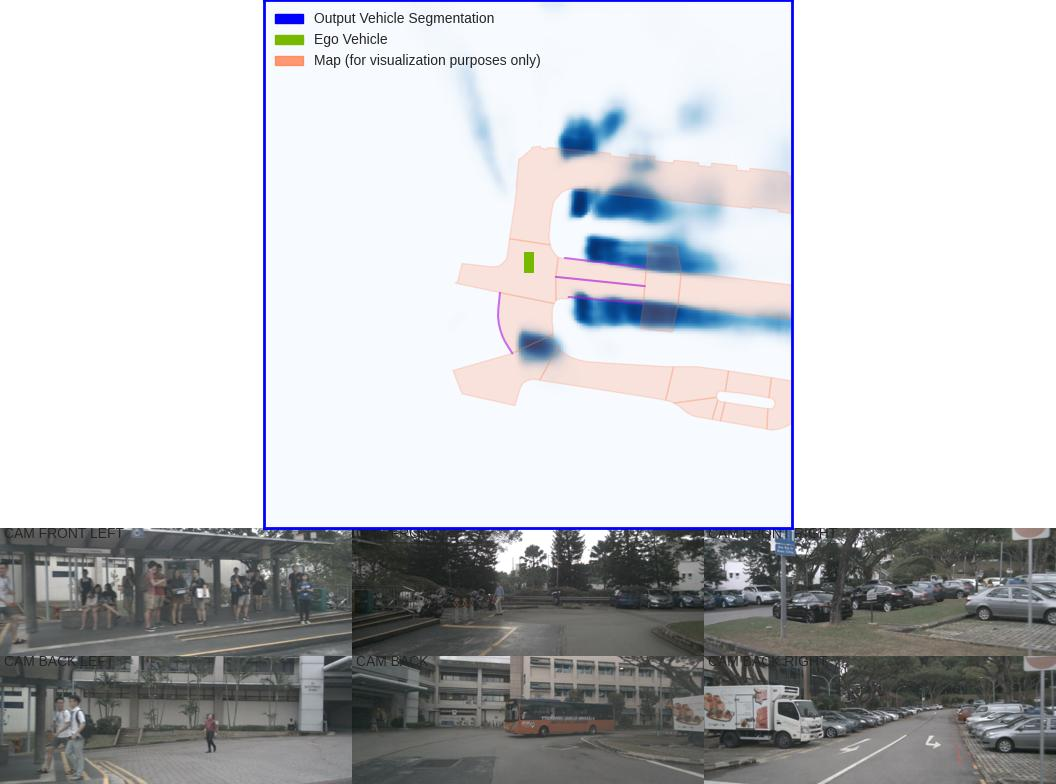
\includegraphics[scale=0.31]{Scriptie/imgs/eval000002_001.jpg}
        \caption{Example of the visualization of the lift-splat algorithm}
        \end{centering}
        \end{figure}


\section*{19 April}
\begin{itemize}
    \item Meeting with Arnoud:
    \begin{itemize}
        \item Alternate between writing the thesis and programming. 
        \item Tobie has a dataset that has different color jerseys for the robots. This can be beneficial for my dataset.
    \end{itemize}
\end{itemize}

\section*{18 April}
Tried to get my own dataset in the algorithm but I currently do not have access to a CUDA gpu. \todo{Did you ask access to a WS to Joey. Do you know which Ubuntu / CUDA version you need?} I can only start testing this with the source code I found on the github repository later (21 april) when I again have access to a CUDA gpu. For now, I can try to implement my own lift-splat algorithm, but I am currently unsure if this is the most efficient way of continuing.  

\section*{14 April}
Downloaded the \href{https://www.nuscenes.org/nuscenes}{NuScenes} dataset to test the Lift-Splat algorithm with to see how it works as the authors intended. With this information I can try to fit in my own dataset into the codebase provided by the authors.
This dataset contains data used for self-driving cars, such as images from pedestrians on sidewalks and other cars. The images also contain labels, which is also possible to provide in my own dataset with the Unity environment.

\section*{13 April}
Found a \href{https://github.com/nv-tlabs/lift-splat-shoot}{github repository} with an implementation of the lift-splat algorithm. Read the code to get an idea of how it works and played around with it a bit. I am going to try and feed it my dataset next.
This repository also allows for multiple visualisations of the model, which can be useful when writing my thesis as it gives the reader a visual representation of the workings of the model.

\section*{12 April}
\begin{itemize}
    \item Made a python notebook to try to visualise the light intensity of the dataset across the field.
        \begin{figure}[!h]
        \begin{centering}
        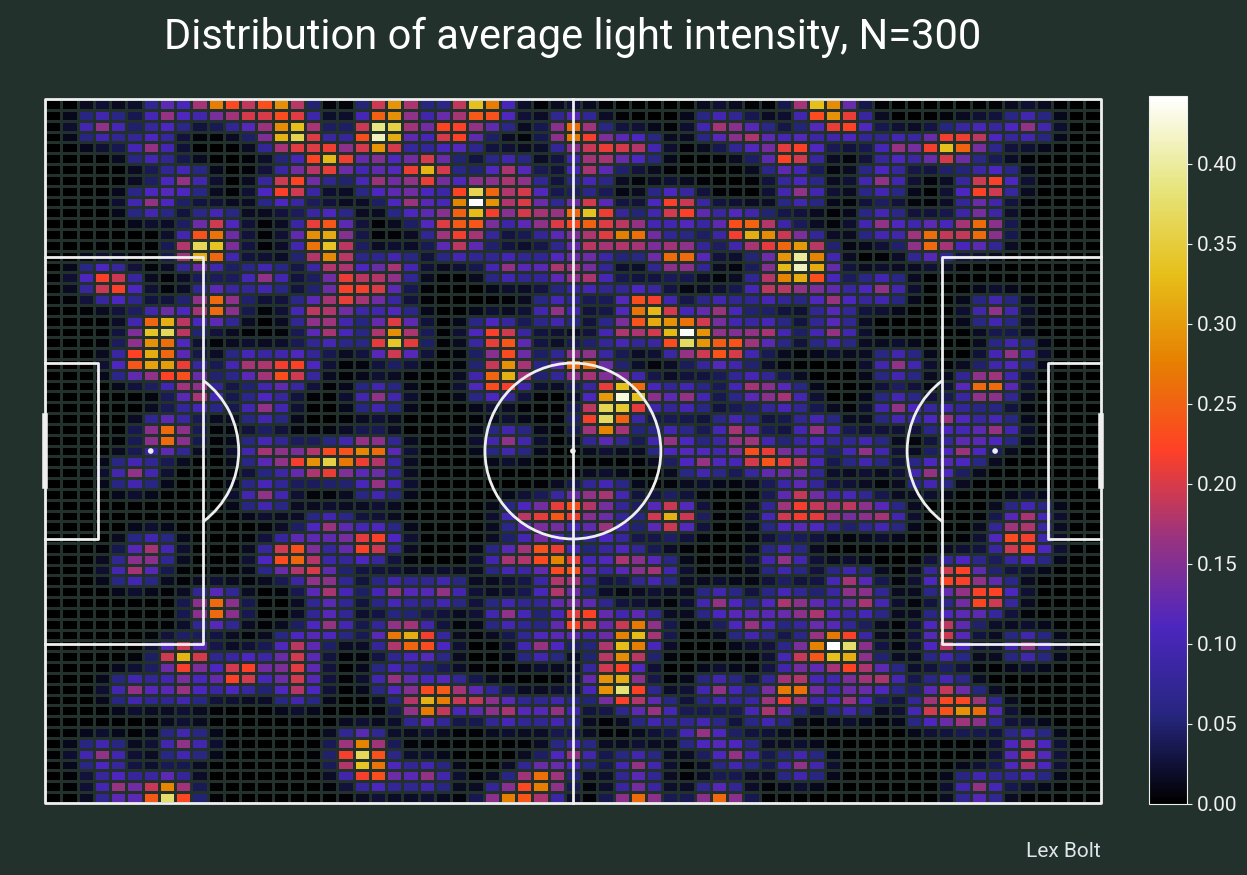
\includegraphics[scale=0.31]{Scriptie/imgs/lightintensity300.png}
        \caption{Screenshot of the light intensity plot by the notebook (n=300)}
        \end{centering}
        \end{figure}

    \item Meeting with Arnoud: 
    \begin{itemize}
        \item Read Xavier's paper about lighting conditions.
        \item For the first draft: focus on the theory and method part. Introduction is of lesser importance for the first draft.
    \end{itemize}
\end{itemize}

\section*{11 April}
\begin{itemize}
\item Generated a dataset with 10.000 entries. This will be my 'programming set'. When I have implemented the lift-splat algorithm and tested the implementation I will generate a larger dataset, and also a dataset with other robots randomly placed on the field.
\item Updated the plot to show a heatmap.
        \begin{figure}[!h]
        \begin{centering}
        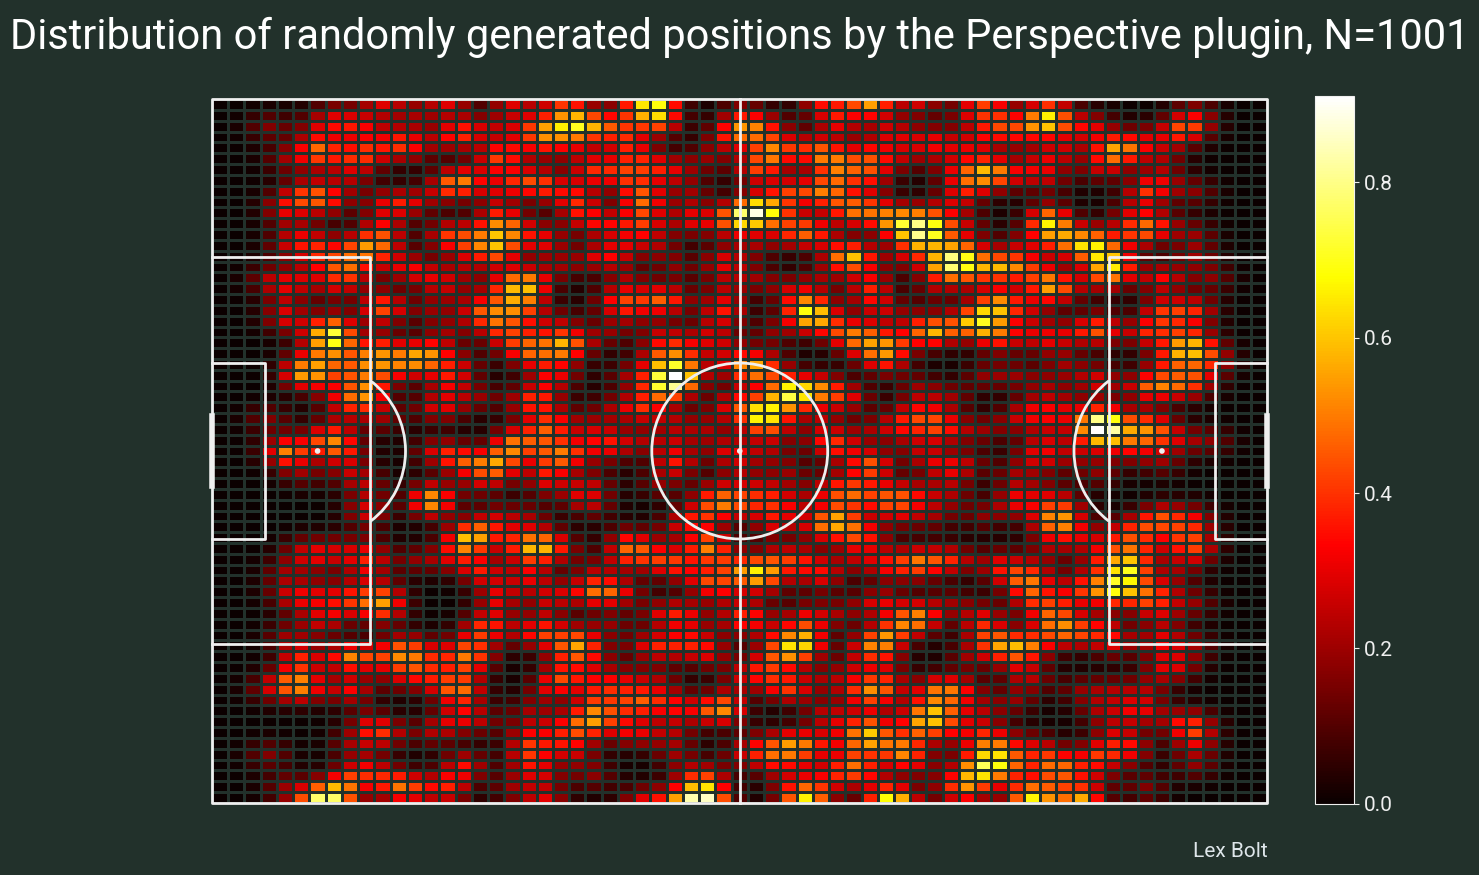
\includegraphics[scale=0.31]{Scriptie/imgs/output.png}
        \caption{Screenshot of the plot by the notebook (n=1001)}
        \end{centering}
        \end{figure}
        As shown in the figure, there are still some 'cold spots' in the distribution. If these persist with a larger dataset I might have to adjust the Perspective settings in order to generate a more even heat map. Looks like the visualisation pays off as it gives me easy insight into the positions of the dataset.
\item Made a python notebook to visualise the location data of a dataset generated by the Unity environment. I made this to prove that a dataset generated by the Unity environment does indeed generate locations with uniform randomness. If the dataset is not uniform, the model can not be trained properly as areas of the field would be missing from the dataset.
        \begin{figure}[!h]
        \begin{centering}
        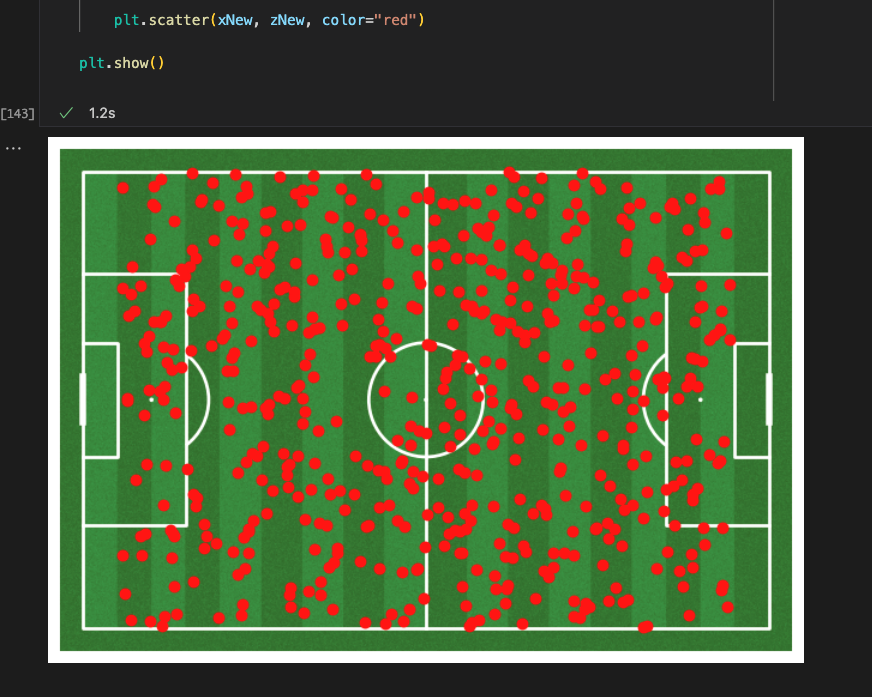
\includegraphics[scale=0.31]{Scriptie/imgs/Screenshot 2023-04-11 at 16.55.10.png}
        \caption{Screenshot of the plot by the notebook (n=600)}
        \end{centering}
        \end{figure}
Note that the above image only has 600 samples. It currently uses a scatterplot, but with datasets of sizes in the thousands this would not be readable anymore. I will change the visualisation to a heatmap later. If the heatmap has roughly the same colour for the entire field, then the random locations were uniformly generated.  

I decided to start working on some visualisation tools as I believe this will help my research further down the line. If I start with making some good testing/visualisation tools now I can have a consisten reference point to compare my progress levels.
\end{itemize}

\section*{7 April}
While reading another paper, I found this quote: "Models trained only on synthetic datasets don’t generalize to real-world data; this phenomenon is called ”domain shift” (Jeon et al., 2021).". I should look further into domain shifts as this could be an important note to make while writing my discussion.
\url{https://arxiv.org/abs/2109.00907}

\section*{6 April}
\begin{itemize}
    \item Incorporated Arnoud's comments on the draft of my project plan into a version that I can hand in on Canvas.
    \item Read Hidde's paper about using GANs in order to generate a background for the robot that more realistically resembles a background that is used in a competitive environment. The results of my paper could be used together with the results of Hidde's paper. Inside of Unity, the backgrounds could be generated with GANs, while the lighting scenario can be randomised with the results of my paper. 
    \item Read Rogier's paper about the obstacle avoidance implementation for the Dutch Nao Team. This paper proposes an obstacle avoidance method that makes use of Dijkstra's shortest path algorithm. The task is to find the lowest cost route through a cost landscape. The peaks in the cost landscape represent obstacles that the robot must avoid, other robots for example. This means that the height map produced by the Lift-Splat algorithm could be used in the obstacle avoidance system, as it could provide a more accurate prediction of where other robots could be on the field. The implementation proposed in the paper only makes use of the YOLOv3 object detection network. 
    \item Arnoud answered my question about the use of the birds-eye view perspective.

\end{itemize}

\section*{5 April}
\begin{itemize}
    \item Read the paper by Jonah Philion and Sanja Fidler about the lift-splat algorithm. This paper will be essential to my research as it describes the algorithm to generate a birds eye view from an image.
    \begin{itemize}
        \item look further into \href{https://single-view-mpi.github.io}{multi plane images} as these are used to generate the point cloud in the lift-splat algorithm.
        \item The paper proposes multiple optimisations that can be useful when I implement my own model.
        \item The 'Lift' part of the algorithm has the goal of lifting each image from a 2D coordinate frame to a 3D coordinate frame. The paper proposes a method of doing this by generating representations at all possible depths for each pixel.
        \item The 'Splat' part of the algorithm uses a \href{https://arxiv.org/abs/1812.05784}{pointpillars} architecture to convert the large point cloud output by the “lift” step into voxels of infinite height (pillars). These pillars are then in a format that can be fed to a CNN.
    \end{itemize}
    \item Worked on the Project Plan that has to be handed in on Friday the 7th of April. The project plan helps me to get an overview of what this thesis want to research. I sent it a draft to Arnoud for feedback.
\end{itemize}


\section*{3 April}

\begin{itemize}
    \item Figured out how to run the Unity scene on my own computer. I am now able to generate my own datasets with randomised parameters for the lighting and robot location. I also connected the camera to the robot so that the robot body will always cast a correct shadow on the field when the camera moves.

    \item Read the Unity Perception by Borkman et al. paper. This paper describes the Unity plugin that I will use to generate the dataset for the model to train on.
    \begin{itemize}
        \item Should look further into the \href{https://github.com/Unity-Technologies/datasetinsights}{DataInsights} python package that the authors of the Unity plugin also made in order to visualise the data generated with the Unity plugin. This python plugin could help to speed up the process of training the position identifying model because it can quickly create an overview of the statistics in the dataset. 
        
    \end{itemize}

    \item Meeting with Arnoud %\todo{Action points?!}
    \begin{itemize}
        \item Start reading the references in the project description and other related articles as soon as possible to get an understanding of the current state of the art.
        \item Fully understand the project's intentions as described in the project description. Make a research question and sub questions based on the current state of the art.
        \item Write an abstract with the \href{http://augmentedtrader.wordpress.com/2012/02/07/8-elements-of-successful-abstracts/}{8 principles of abstracts}.
        \item Get familiarised with the controls of Unity, how to interface with Unity using C\#.
        \item Try to get the camera into/attached to the robot so the model of the robot moves when the camera's position is randomised. This will cause the shadow of the robot to also be in frame, which will be a constant factor when testing the end result with actual data.
        \item Note: If the sunlight always comes from the same window, a model might over train on the shadows being on one 'compass line'.
        \item Make a project planning before Friday. Preferably earlier to get feedback from Arnoud.
    \end{itemize}
\end{itemize}

\end{document}
    